\documentclass{tufte-handout}

\title{An Introduction to STAMP Safety Analysis}
\author[Kep Peterson]{Kep Peterson}

%\geometry{showframe} % display margins for debugging page layout

\usepackage{graphicx} % allow embedded images
  \setkeys{Gin}{width=\linewidth,totalheight=\textheight,keepaspectratio}
  \graphicspath{{/graphics/}} % set of paths to search for images
\usepackage{amsmath}  % extended mathematics
\usepackage{booktabs} % book-quality tables
\usepackage{units}    % non-stacked fractions and better unit spacing
\usepackage{multicol} % multiple column layout facilities
\usepackage{lipsum}   % filler text
\usepackage{fancyvrb} % extended verbatim environments
\fvset{fontsize=\normalsize}% default font size for fancy-verbatim environments
\usepackage{graphicx}
\graphicspath{ {../images/} }

% Standardize command font styles and environments
\newcommand{\doccmd}[1]{\texttt{\textbackslash#1}}% command name -- adds backslash automatically
\newcommand{\docopt}[1]{\ensuremath{\langle}\textrm{\textit{#1}}\ensuremath{\rangle}}% optional command argument
\newcommand{\docarg}[1]{\textrm{\textit{#1}}}% (required) command argument
\newcommand{\docenv}[1]{\textsf{#1}}% environment name
\newcommand{\docpkg}[1]{\texttt{#1}}% package name
\newcommand{\doccls}[1]{\texttt{#1}}% document class name
\newcommand{\docclsopt}[1]{\texttt{#1}}% document class option name
\newenvironment{docspec}{\begin{quote}\noindent}{\end{quote}}% command specification environment

\geometry{
  %left=.5in,
  %right=.5in,
  %top=.5in,
  bottom=.5in
}

\title{Toolkit: Control Loop With Causal Factors}

\begin{document}

\setlength{\parindent}{0em}
\setlength{\parskip}{.75em}

%\maketitle

%\tableofcontents

%\bibliography{sample-handout}
%\bibliographystyle{plainnat}

\section{Control Loop With Causal Factors}

This diagram shows common flaws in a control loop, or \textbf{causal factors}, that might contribute to the controller misapplying an action or failing to take an action it should have, which we identify as an \textbf{unsafe control action} if it results in a \textbf{hazard}. We use this diagram to guide our brainstorming about why each \textbf{unsafe control action} might occur, identifying \textbf{causal scenarios} we can design features to prevent.

\begin{fullwidth}
\begin{center}
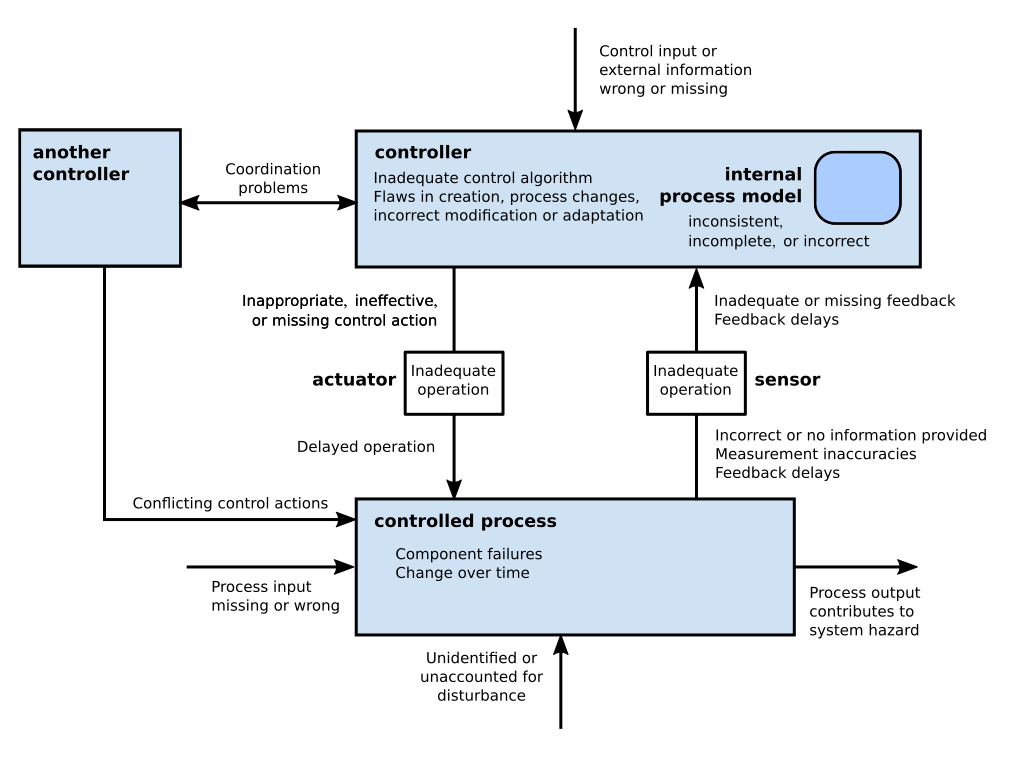
\includegraphics[width=4in]{../images/generic_control_loop-flaws.png}
\end{center}
\end{fullwidth}

[Based on a diagram from \emph{Engineering A Safer World} p.223]

\end{document}
